\documentclass[12pt]{article}
\usepackage[spanish]{babel}
\usepackage{graphicx}
\usepackage[margin=1in]{geometry}
\usepackage[utf8]{inputenc}


\begin{document}
	\begin{titlepage}
		\centering
		{
\includegraphics[width=0.2\textwidth]{img/Logo}\par}
		\vspace{1cm}
		{\bfseries\LARGE Universidad del Valle \par}
		\vspace{1cm}
		{\scshape\Large PROGRAMA DE INGENIERÍA DE SISTEMAS  \par}
		\vspace{1.5cm}
		{\scshape\Huge Laboratorio 1 \par}
		\vspace{1.5cm}
		{\itshape\Large Probabilidad y Estadística \par}
		\vfill
		{\Large Integrantes: \par}
		{\Large Maycol Andres Taquez Carlosama \textbf{2375000} \par}
		{\Large Santiago Valencia Aguiño \textbf{2343334} \par}
		\vfill
		{\Large Docente: \par}
		{\Large Gabriel Conde Arango \par}
		\vfill
		{\Large Abril 2025 \par}
	\end{titlepage} \newpage
	\tableofcontents
	\newpage
	\section{Descripción}  
	Una compañía le ha encargado a usted que la asesore en la decisión sobre cuáles bolsas de 5g de azúcar debe 
	comprar. Su tarea es evaluar si el contenido de azúcar en bolsas pequeñas es de 5g, como se anuncia en su 
	etiqueta. Se dispone de bolsas de azúcar de dos productores. 
	
	\section{Actividad}
	
	\subsection{¿Cuántas poblaciones hay en este problema? ¿Cuáles son? }
	En el problema hay dos poblaciones, ya que se están estudiando los paquetes de azúcar de dos empresas azucareras \textbf{Manuelita} e \textbf{Incauca}.
	
	\subsection{¿Cuáles son las variables de interés en este estudio? ¿Cuáles son las escalas de medición?}
	Las variables de estudio son el peso de los paquetes con azúcar, el peso solo del azúcar y el peso de las bolsas vacías, de ambas empresas, usando como medición los \textbf{gramos}. Estos datos fueron tomados en el laboratorio del edificio de Estadística, usando una balanza digital. En el proceso se tomo muestras de 16 de paquetes de 5 gramos, de cada empresa, el margen de error de cada medición no se pudo tomar con exactitud debido a que la balanza solo mostraba dos cifras significativas para cada medición. 
	
	\subsection{¿Está cumpliendo cada una de estas empresas su ofrecimiento de empacar 5g de azúcar en cada bolsa?}
	Para determinar si cada empresa empaca 5g de azúcar en cada bolsa se ha decidido tomado en cuenta la columna de datos Peso de azúcar.
	Como los datos obtenidos son de naturaleza cuantitativa continua se ha hecho la siguiente Tabla de frecuencias del azúcar sin su bolsa.
	
	\begin{table}[h!]
		\centering
		\begin{tabular}{|c|c|c|c|c|c|}
			\hline
			\textbf{Intervalo} & \textbf{Frec\_Abs} & \textbf{Frec\_Rel} & \textbf{Frec\_Acum} & \textbf{Frec\_Rel\_Acum} \\
			\hline
			$[4.6, 4.8)$ & 1 & 0.0625 & 1 & 0.0625 \\
			\hline
			$[4.8, 5)$ & 4 & 0.2500 & 5 & 0.3125 \\
			\hline
			$[5, 5.2]$ & 11 & 0.6875 & 16 & 1.0000 \\
			\hline
		\end{tabular}
		\caption{Tabla de frecuencias-Peso de Azucar-Empresa Manuelita}
	\end{table}
	
	\begin{table}[h!]
		\centering
		\begin{tabular}{|c|c|c|c|c|c|}
			\hline
			\textbf{Intervalo} & \textbf{Frec\_Abs} & \textbf{Frec\_Rel} & \textbf{Frec\_Acum} & \textbf{Frec\_Rel\_Acum} \\
			\hline
			$[4.6,4.73)$ & 1 & 0.0625 & 1 & 0.0625 \\
			\hline
			$[4.73,4.87)$ & 6 & 0.3750 & 7 & 0.4375 \\
			\hline
			$[4.87,5]$ & 9 & 0.5625 & 16 & 1.0000 \\
			\hline
		\end{tabular}
		\caption{Tabla de frecuencias-Peso de Azucar-Empresa Incauca}
	\end{table}
	
	Con los anteriores tablas, se puede sacar la siguiente información: \\
	\vspace{0.2cm}
	
	\textbf{{\large Medidas de centralidad y dispersión para la Fabrica Manuelita}}\\
	{\large Media:} 4.93 \\
	{\large Desviación estándar:} 0.14 \\
	{\large Coeficiente de variación}: $2.83\%$ \\
	\vspace{0.2cm}

	\textbf{{\large Medidas de centralidad y dispersión para la Fabrica Incauca}} \\
	{\large Media:} 4.9 \\
	{\large Desviación estándar:} 0.126 \\
	{\large Coeficiente de variación}: $2.57\%$ \\
	\vspace{0.2cm}
	
	{\large \textbf{Conclusión}}: 
	Aunque los valores son muy pequeños se puede decir que las empresas no ofrecen un empaquetado preciso de $5g$ de azúcar, esto se ve reflejado en las medidas de centralidad obtenidas de ambas empresas, para la Fabrica Manuelita, la media es de 4.93 lo cual indica que los datos no se concentran en 5, y lo mismo sucede con la Fabrica Incauca, cuya media es de 4.9, que está alejada un poco más del valor ideal. Además la medida de dispersión como el coeficiente de variación $CV$ permite corroborar nuestra conclusión indicando que los datos no son homogéneos. Si los datos no estuvieran dispersos, su  $CV$ sería del $0.0\%$
	
	\subsection{¿Son mayores las cantidades de azúcar empacadas en las bolsas de una empresa que en las de la otra? }
	Teniendo en cuenta que solo se está midiendo el azúcar sin el empaque, entonces se debe recurrir a otras herramienta pues las medidas obtenidas como la media $\overline{x}$ y el  $CV$ en la anterior pregunta no nos permiten llegar a una respuesta.\\
	
	La función empírica de frecuencia relativa acumulada $P(X\le x)$, nos permite realizar el siguiente analisis.
	\vspace{0.2cm}
	
	\textbf{{\large Fabrica Manuelita}}\\
	$P(X<5) = 31.25\%$ \\
	$P(X>5) = 6.25\%$ \\
	\vspace{0.2cm}
	
	\textbf{{\large Fabrica Incauca}}\\
	$P(X>5) = 43.75\%$ \\
	$P(X>5) = 0\%$ \\
	
	Aunque el coeficiente de variación de la fabrica Manuelita es mayor que el de su competencia, esto no permite decir nada de cual empresa ofrece una mayor cantidad de azúcar empacada. Pero con la función empírica de frecuencia relativa acumulada se puede determinar lo siguiente.
	
	El $31.25\%$ de los empaques de la fabrica Manuelita tiene un peso menor a $5 gramos$, mientras que en la fabrica Incauca el  $43.75\%$, de sus empaques tienen un peso menor que a $5 gramos$.
	En \textbf{conclusión} la fabrica Manuelita ofrece mayores cantidades de azúcar de empacado en las bolsas. 
	
	Lo anterior se puede visualizar graficamente con las siguientes funciónes de densidad. \\
	
	
	\begin{figure}[ht]
		\centering 
		\begin{minipage}{0.45\textwidth} 
			\centering
			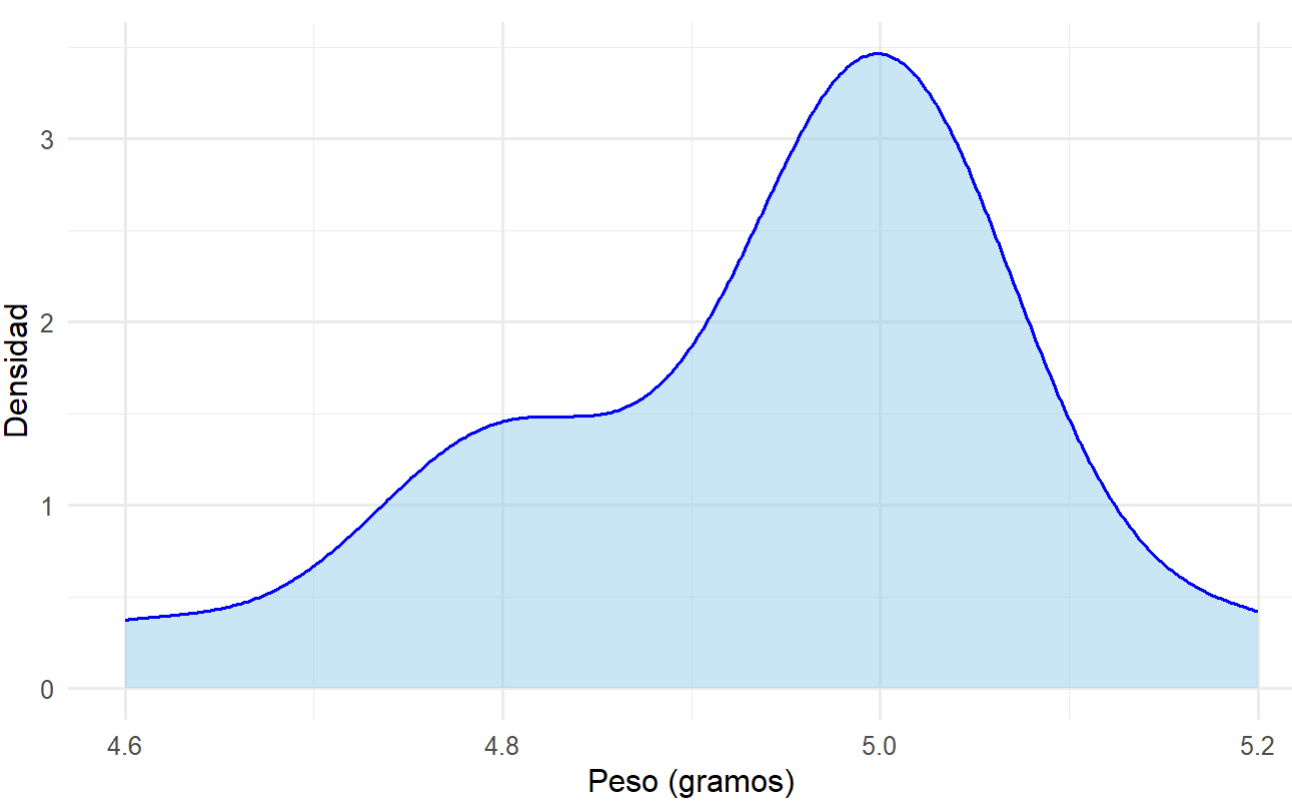
\includegraphics[width=\linewidth]{img/densidad1} 
			\caption{Función de densidad de la fabrica Manuelita} 
			\label{fig:densidad1}
		\end{minipage}
		\hfill 
		\begin{minipage}{0.45\textwidth} 
			\centering
			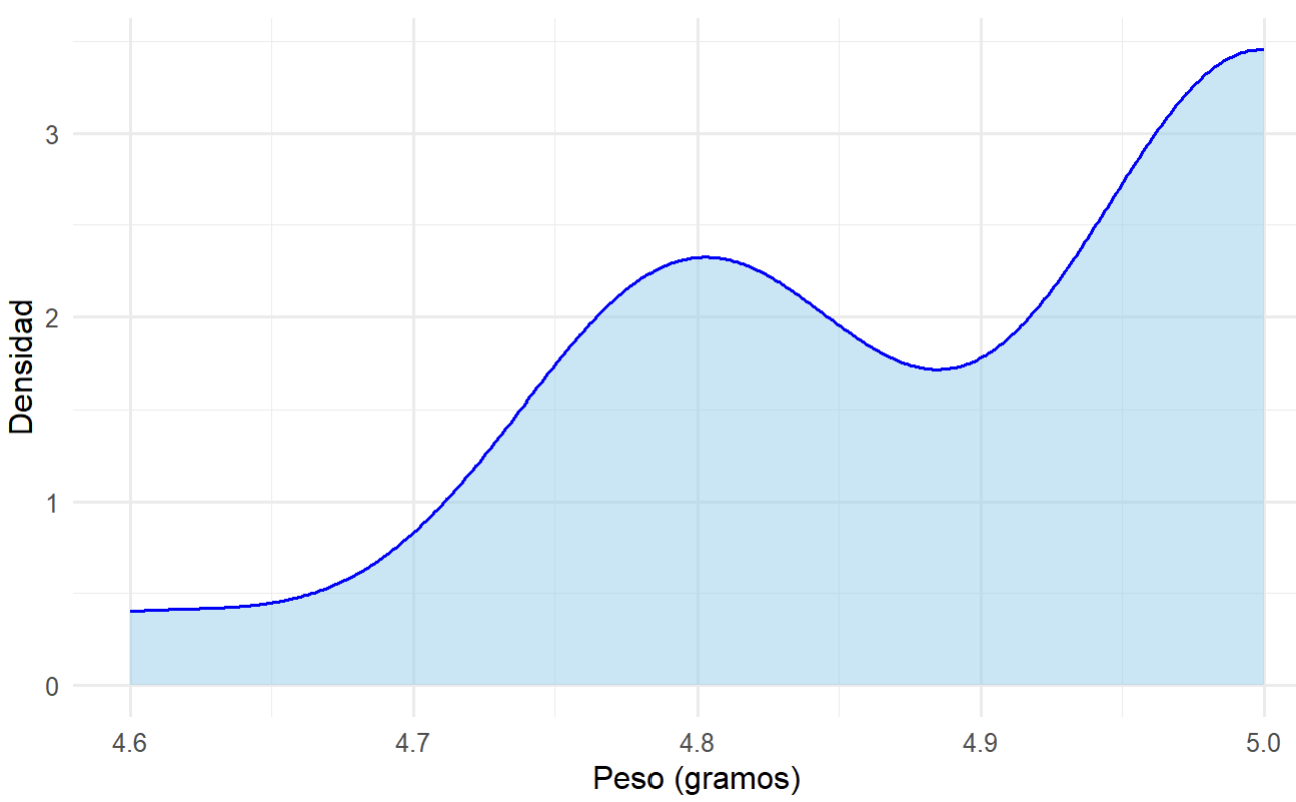
\includegraphics[width=\linewidth]{img/densidad2}
			\caption{Función de densidad de la fabrica Incauca}
			\label{fig:densidad2}
		\end{minipage}
	\end{figure}
	
	\subsection{¿Son las bolsas vacías de una empresa más pesadas que las de la otra? }
	Para ello se ha decidido obtener otra columna de datos llamada \textbf{"Peso de Bolsas"}, la cual se obtiene a partir de la diferencia de los datos de la columna \textbf{"Peso de Bolsa Sellada"} y \textbf{"Peso de Azucar"}. 
	
	Los datos obtenidos son los siguientes:\\ 
	
	\begin{table}[h!]
		\centering
		\begin{tabular}{|c|c|c|c|} 
			\hline
			0.1 & 0.1 & 0.1 & 0.1 \\ 
			\hline
			0.2 & 0.2 & 0.2 & 0.2 \\ 
			\hline
			0.2 & 0.2 & 0.2 & 0.4 \\ 
			\hline
			0.4 & 0.4 & 0.4 & 0.6 \\ 
			\hline
		\end{tabular}
		\caption{Peso de bolsas vacias-Empresa Manuelita}
	\end{table} \newpage
	
	\begin{table}[h!]
		\centering
		\begin{tabular}{|c|c|c|c|} 
			\hline
			0.1 & 0.2 & 0.2 & 0.2 \\ 
			\hline
			0.2 & 0.2 & 0.2 & 0.4 \\ 
			\hline
			0.4 & 0.4 & 0.4 & 0.6 \\ 
			\hline
			0.6 & 0.6 & 0.6 & 0.6 \\ 
			\hline
		\end{tabular}
		\caption{Peso de bolsas vacias-Empresa Incauca}
	\end{table}
	
	A partir de los datos directamente se obtienen las siguientes métricas. \\
	
	\textbf{{\large Medidas de centralidad y dispersión para la Fabrica Manuelita}}\\
	{\large Media:} 0.25 \\
	{\large Desviación estándar:} 0.14 \\
	{\large Coeficiente de variación}: $56\%$ \\
	\vspace{0.2cm}
	
	\textbf{{\large Medidas de centralidad y dispersión para la Fabrica Incauca}}\\
	{\large Media:} 0.34 \\
	{\large Desviación estándar:} 0.178 \\
	{\large Coeficiente de variación}: $52.01\%$ \\
	\vspace{0.2cm}
	
	{\large \textbf{Conclusión}}: 
	Tomando como referencia la media, la empresa Manuelita tiene una media de $\overline{x_1}=0.25g$ que es menor, con respecto a la fabrica Incauca $\overline{x_2}=0.34g$, lo que indica que la fabrica Incauca tiene bolsas vacías con mayor peso, pero estas medidas varian mucho con respecto a su media, eso es lo que indica su coeficiente de variación. 
	
	Por otro lado la empresa Incauca, tiene menor variabilidad con respecto a su competencia pero no por eso deja de tener datos muy heterogéneos. 
    \vspace{0.5cm}
	Por lo que se concluye que la empresa Icauca tiene bolsas vacias más pesadas. Esto puede ser un buen indicador ya se porque tiene más grosor o calidad del material, pero solo es una hipotesis.

    \subsection{¿Cuál proveedor le recomendaría a la gerencia de la compañía? ¿Por qué?}

Para determinar la recomendación del proveedor se analizarán detalladamente los datos disponibles, examinando tanto las variables numéricas como las no numéricas para comprender la estructura y calidad de la información. Se aplicarán técnicas estadísticas y se utilizarán herramientas gráficas, como los diagramas de cajas, para visualizar la distribución de los indicadores clave, identificando patrones, variabilidad y valores atípicos.  

\vspace{0.5cm}
Este análisis se complementará con el cálculo de medidas de tendencia central y dispersión, lo que permitirá comparar objetivamente el desempeño de cada proveedor. La integración de estos enfoques garantizará que la decisión final se base en criterios estadísticos sólidos y en una evaluación integral de la consistencia y predictibilidad de los datos.

\begin{figure}[ht]
    \centering 
    \begin{minipage}{0.45\textwidth} 
        \centering
        \includegraphics[width=\linewidth]{img/diagr_caja_N°1.png} 
        \caption{Diagrama de caja - Peso de azúcar por empresa} 
        \label{fig:boxplot_azucar}
    \end{minipage}
    \hfill 
    \begin{minipage}{0.45\textwidth} 
        \centering
        \includegraphics[width=\linewidth]{img/diagr_caja_N°2.png}
        \caption{Diagrama de caja - Peso de bolsas vacías por empresa}
        \label{fig:boxplot_bolsas}
    \end{minipage}
\end{figure}

\newpage

\textbf{Interpretación del diagrama de caja - Peso de azúcar:}
\begin{itemize}
    \item \textbf{Manuelita:} El diagrama de caja abarca de 4.8 a 5.0, con la mediana en 5.0. Valor atípico: 5.2g (por encima del límite superior).
    \item \textbf{Incauca:} El diagrama de caja abarca de 4.8 a 5.0, con la mediana en 5.0. Valor atípico: 4.6g (por debajo del límite inferior).
    \item Ambas empresas tienen medias cercanas a 5g, pero Manuelita muestra un valor atípico por encima de 5g (5.2g), mientras que Incauca tiene un Valor atípico por debajo (4.6g). La dispersión (IQR = 0.2) es igual en ambas, pero Manuelita tiene un rango total mayor (4.6-5.2 vs. 4.6-5.0).
\end{itemize}

\begin{table}[h!]
    \centering
    \begin{tabular}{|c|c|c|}
        \hline
        \textbf{Métrica} & \textbf{Manuelita} & \textbf{Incauca} \\
        \hline
        Mínimo & 4.6 & 4.6 \\
        Primer Cuartil (Q1) & 4.8 & 4.8 \\
        Mediana (Q2) & 5.0 & 5.0 \\
        Tercer Cuartil (Q3) & 5.0 & 5.0 \\
        Máximo & 5.2 & 5.0 \\
        Rango Intercuartílico IQR (Q3 - Q1) & 0.2 & 0.2 \\
        Límite Inferior & \(4.8 - 1.5 \times 0.2 = 4.5\) & \(4.8 - 1.5 \times 0.2 = 4.5\) \\
        Límite Superior & \(5.0 + 1.5 \times 0.2 = 5.3\) & \(5.0 + 1.5 \times 0.2 = 5.3\) \\
        Valores atípicos & 5.2 \,(\text{superior}) & 4.6 \,(\text{inferior}) \\
        \hline
    \end{tabular}
    \caption{Resumen estadístico - Peso de azúcar (gramos)}
    
\end{table}


\textbf{Interpretación del diagrama de caja - Bolsas vacías:}
\begin{itemize}
    \item \textbf{Manuelita:} Caja de 0.2 a 0.4, mediana en 0.2. Valor atípico: 0.6g (por encima del límite superior).
    \item \textbf{Incauca:} Caja de 0.2 a 0.6, mediana en 0.4. Sin valores atípicos.
    \item Incauca tiene bolsas más pesadas (mediana = 0.4g vs. 0.2g) y mayor dispersión (IQR = 0.4). Manuelita muestra un valor atípico en 0.6g, indicando inconsistencia en el peso de sus bolsas.
\end{itemize}

\begin{table}[h!]
    \centering
    \begin{tabular}{|c|c|c|}
        \hline
        \textbf{Métrica} & \textbf{Manuelita} & \textbf{Incauca} \\
        \hline
        Mínimo & 0.1 & 0.2 \\
        Q1 & 0.2 & 0.2 \\
        Mediana (Q2) & 0.2 & 0.4 \\
        Q3 & 0.4 & 0.6 \\
        Máximo & 0.6 & 0.6 \\
        Rango Intercuartílico IQR & 0.2 & 0.4 \\
        Límite Inferior & \(0.2 - 1.5 \times 0.2 = -0.1\) & \(0.2 - 1.5 \times 0.4 = -0.4\) \\
        Límite Superior & \(0.4 + 1.5 \times 0.2 = 0.7\) & \(0.6 + 1.5 \times 0.4 = 1.2\) \\
        Valores atípicos & 0.6 \,(\text{superior}) & Ninguno \\
        \hline
    \end{tabular}
    \caption{Resumen estadístico - Peso de bolsas vacías (gramos)}
\end{table}

{\large \textbf{Conclusión}}:  
Aunque Manuelita tiene una media de azúcar ligeramente superior, Incauca destaca por su menor variabilidad (CV) en el peso del azúcar y mayor consistencia en el peso de las bolsas vacías. Dado que ninguna empresa cumple plenamente con los 5g, se prioriza la consistencia sobre la cercanía al valor ideal, ya que esto refleja un proceso de producción más controlado y predecible.  

\vspace{0.5cm} 
\textbf Seleccionar a Incauca, exigiendo ajustes para alcanzar los 5g, dado que su menor dispersión facilita correcciones técnicas.
	
\end{document}